\documentclass{article}
\usepackage[utf8]{inputenc}
\usepackage[a4paper, total={6in, 8in}, margin = 3cm]{geometry}
\usepackage[english]{babel}
\usepackage{authblk}
\usepackage{enumitem}
\usepackage{mathtools}
\usepackage{amssymb}
\usepackage{amsmath}
\usepackage{setspace}
\usepackage{natbib}
\usepackage{subfigure}
\usepackage{todonotes} % for comments


\newcommand{\ziang}{\textcolor{blue}}


\title{\textbf{Bayesian smoothing with extended second order random walk model: An detailed overview and comparison}}

\author{
Ziang Zhang \\ \vspace{-0.3cm}\normalsize\texttt{aguero.zhang@mail.utoronto.ca}\\ 
\large
\vspace{0.5cm}
Supervisor(s): James Stafford, Patrick Brown \\ 

\vspace{0.5cm}
Department of Statistical Sciences \\
University of Toronto
}

\date{June 2021}

\doublespacing


\begin{document}


\maketitle

\tableofcontents

\newpage

\begin{abstract}
In this report, we will describe and implement the extended second order random walk model proposed in \cite{rw2}. This method can be viewed as an extension of the formerly used second order random walk model to irregular spaced locations/knots, derived from discretizing a stochastic differential equation. We will compare this method with other Bayesian smoothing spline methods, both conceptually and practically. This report will provide practitioners with a more thorough understanding of the connection between the second order random walk model and other Bayesian smoothing methods, and a practical guideline on how to choose among these methods.
\end{abstract}




\section{Introduction}\label{intro}

Smoothing methods are often used when there is little information on the functional structures of some covariate effects. The main challenging of smoothing is to provide enough flexibility so that the functional form of covariate effect can be accurately inferred without over-fitting the observed data. In smoothing spline method, this trade off is controlled by a smoothing parameter $\lambda$, which penalizes the wiggliness of inferred function. 

Consider a data set $\{y_i,x_i, i\in [n]\}$, and a nonparametric model $y_i = g(x_i) + \epsilon_i$ where $\epsilon_i \overset{iid}\sim N(0,\sigma_\epsilon^2)$ and $x_i \in [a,b]$, then the smoothing spline aims to solve the following problem:
\begin{equation}\label{equ:ss}
\arg\min_{g\in C^2} \bigg\{ \sum_i\bigg(y_i-g(x_i)\bigg)^2 + \lambda\int_a^b g''(x)^2 dx \bigg\}
\end{equation}
The sum of square term on the left can be replaced by negative log likelihood, which is also called \textit{penalized likelihood} method.

In typical frequentist method, the smoothing parameter $\lambda$ is either taken as fixed value input by the users, or substituted by an optimal value selected from procedure such as REML. Therefore, how to take into account the uncertainty with the unknown hyper-parameter increases the difficulty of frequentist smoothing methods. On the other hand, the hyper-parameter $\lambda$ will be assigned with a prior distribution in Bayesian smoothing methods, and hence any uncertainty involved with that parameter will be taken into account for the inference. Furthermore, the development of approximate Bayesian inference methods such as \cite{inla} enables Bayesian smoothing to be implemented in a computationally convenient way. Hence, application of Bayesian smoothing method can be advantageous in a lot of settings.


Based on the well known connection between smoothing splines and integrated Wiener processes \citep{wahba}, \cite{rw2} developed a Bayesian smoothing method by assigning a stochastic differential equation (SDE) based prior to the unknown true effect functions. 
Their method uses a finite element method called Galerkin approximation to the SDE, and then solves for its weak solution. Therefore, the method of \cite{inla} can be viewed as an extension of the second order random walk model (RW2) to irregular spaced locations.
The hyper-parameter $\sigma_s$ which is defined as $\sigma_s \propto 1/\lambda$, represents the standard deviation parameter of the second derivative of the covariate effect function, and will be assigned with a proper prior distribution. Because of the use of numerical approximation, the resulting prior distribution for the effect function will have a sparse precision matrix, and hence will be computationally efficient if used together with approximate Bayesian inference method such as Integrated Nested Laplace Approximation (INLA) \citep{inla}. Both theoretical results and simulation results have been demonstrated for their Galerkin approximation methods in their original paper \citep{rw2}.


In section \ref{SmoothSpline}, we will describe how is smoothing spline typically fitted in Frequentist method, and how it can be reinterpreted as an equivalent Bayesian inference problem with ARIMA prior when locations are equally spaced \citep{ARIMA}. In section \ref{rw2}, we will introduce the extended second order random walk method proposed in \cite{rw2}, and provide conceptual comparison and connection with the the exact method using ARIMA method. Furthermore, we will write the ARIMA method in the form of a similar SDE specification, and hence generalize the ARIMA method to irregular spaced locations and enhances its computational efficiency. In section \ref{practice}, we will implement several simulation studies to illustrate the differences between all the mentioned Bayesian smoothing spline methods, in aspects of prior sensitivity, inference accuracy and computational efficiency. We conclude in section \ref{conclusion} with a discussion.


\section{Smoothing Spline}\label{SmoothSpline}

\subsection{Fitting Smoothing Spline}

Consider the smoothing parameter $\lambda$ in equation \ref{equ:ss} is a fixed constant, the solution to the \textit{penalized likelihood} equation \ref{equ:ss}, denoted as $\hat{g}_\lambda(.)$, is well known to be a natural cubic polynomial spline when the response variable $\boldsymbol{y}:= (y_1, y_2, ..., y_n)^T \in \mathbb{R}^n$ cannot be perfectly interpolated by a lower order polynomial function. For any function $g$, let $\boldsymbol{g} := (g(x_1), ..., g(x_n))^T \in \mathbb{R}^n$ denotes the corresponding evaluation vector, then the solution cubic spline $\hat{g}_\lambda(.)$ can be uniquely determined based on its evaluation vector $\boldsymbol{\hat{g}_\lambda}$ \citep{smoothingspline}. 



Using the property of natural cubic spline, the term $\int_a^b g''(x)^2 dx$ for any natural cubic spline $g(.)$ can be written as $\boldsymbol{g}^T K \boldsymbol{g}$, where the matrix $K$ only depends on the covariate locations $\boldsymbol{x} := (x_1, ..., x_n)^T \in \mathbb{R}^n$, not on the response variable $\boldsymbol{y}$. Therefore, the equation \ref{equ:ss} in section \ref{intro} can be written in the following vector form:
\begin{equation}\label{equ:vectorss}
\arg\min_{\boldsymbol{g}\in \mathbb{R}^n}(\boldsymbol{y} - \boldsymbol{g})^T (\boldsymbol{y} - \boldsymbol{g}) + \lambda \boldsymbol{g}^T K \boldsymbol{g}.
\end{equation}
Since this function is convex in $\boldsymbol{g}$, taking derivative and setting it to zero yields the evaluation vector $\boldsymbol{\hat{g}_\lambda} = (I+\lambda K)^{-1} \boldsymbol{y}$. Hence the solution function can be recovered from this evaluation vector. 

The above procedures all treat the single smoothing parameter $\lambda$ as a fixed constant. In practice, there are two common ways to select the value of $\lambda$: selecting a constant based on the subjective belief on the required smoothness of the fitted function or estimating its value based on the observed data \citep{smoothingspline}. 

If one decides to estimate the smoothing parameter using the same set of data, methods such as cross-validation (CV), generalized cross-validation(GCV) or restricted maximum likelihood estimation (REML) can be used. When computing quantities such as confidence intervals and standard errors, traditional frequentist approaches will directly plug in the estimate of $\lambda$ and treat it as a known value. Therefore the traditional frequentist inference methods will tend to underestimate the variability, because they ignore the additional uncertainty from the estimation of $\lambda$. For this reason, Bayesian smoothing methods which fully take into account the uncertainty with the value of $\lambda$ can be preferred at many applications.










\subsection{Bayesian Smoothing Spline with ARIMA Model}

Besides the frequentist penalized likelihood interpretation, the smoothing spline can also be interpreted as a Bayesian inference problem with partially diffuse priors \citep{ARIMA}. Recall in the vectorized (negative) penalized likelihood equation \ref{equ:vectorss}, the first term can be regarded as the (negative) log likelihood $\log f(\boldsymbol{y}|\boldsymbol{g},\lambda)$, and the second term can be viewed as the (negative) log prior for $\boldsymbol{g}$, denoted as $\log f(\boldsymbol{g})$. If we assume the smoothing parameter $\lambda$ is a known constant, then equation \ref{equ:vectorss} can be interpreted as (negative) log joint likelihood $\log f(\boldsymbol{y},\boldsymbol{g})$ which has the same maximum $\hat{\boldsymbol{g}}$ as the log posterior $\log f(\boldsymbol{g}|\boldsymbol{y})$.

The likelihood above corresponds to $\boldsymbol{y}|\boldsymbol{g} \sim N(0, I)$, and the prior for $\boldsymbol{g}$ corresponds to $\boldsymbol{g} \sim N(0, \frac{1}{\lambda} K^{-1})$. The implicit assumption that $\sigma_\epsilon = 1$ here is not stringent, as one can easily reparametrize the parameter $\lambda$ as $\frac{\lambda}{\sigma_\epsilon^2}$ without changing the shape of the posterior for $\boldsymbol{g}$.
To better understand the prior for $\boldsymbol{g}$, note that the precision matrix $K$ can be factorized as the following:
\begin{equation}\label{equ:ArimaPrior}
K = D^T R^{-1} D.
\end{equation}
When all the locations are equally spaced with unit spacings, the $(n-2) \times n$ matrix $D$ will be the second order difference matrix defined as:
\begin{equation}
\begin{aligned}
D = \mbox{\scriptsize $\begin{bmatrix}
1 & -2 & 1 & 0 & 0 & \cdots & 0\\
0 & 1 & -2 & 1 & \cdots & 0 & 0\\
0 & \vdots &  &  & \ddots & 0 & 0\\
0 & 0 & 0 & \cdots & 1 & -2 & 1\\
\end{bmatrix}$}
\end{aligned},
\end{equation}

and the $(n-2) \times (n-2)$ matrix R is a strictly positive definite matrix that can be computed as:
\begin{equation}
\begin{aligned}
R = \mbox{\scriptsize $\begin{bmatrix}
\frac{2}{3} & \frac{1}{6} & 0 & 0 & 0 & \cdots & 0\\
\frac{1}{6} & \frac{2}{3} & \frac{1}{6} & 0 & 0 & \cdots & 0\\
0 & \frac{1}{6} & \frac{2}{3} & \frac{1}{6} & 0 & \cdots & 0\\
 &  &  &  &  & \ddots & \\
0 & 0 & 0 & \cdots & 0 & \frac{1}{6} & \frac{2}{3}\\
\end{bmatrix}$}
\end{aligned}.
\end{equation}

Note that the $D$ matrix can be viewed as a second order difference operator, that functions on the evaluation vector $\textbf{g}$ to get its second order difference vector $\boldsymbol \gamma := D \boldsymbol g$. Hence $\boldsymbol g^TK \boldsymbol g$ can be equivalently computed as $\boldsymbol \gamma^T R^{-1} \boldsymbol \gamma$. In other words, if we define $\sigma_s^2 := \frac{1}{\lambda}$, adding the penalty term is equivalent to assigning a prior to the second order difference vector $\boldsymbol \gamma \sim N(0,\sigma_s^2R)$.

Let $\boldsymbol \gamma:=(\gamma_3,...,\gamma_n)^T \in \mathbb{R}^{n-2}$, with $\gamma_i :=g(x_i)-2g(x_{i-1})+g(x_{i-2})$, then we can notice that the covariance matrix $R$ of $\boldsymbol \gamma$ has the same structure as a MA(1) model. Let $\boldsymbol \xi :=(\xi_2,...,\xi_n)^T \sim N(0, I)$, and define $\gamma_i = \theta\xi_{i-1} +\xi_i$, then we can write $\boldsymbol \gamma = \Theta \boldsymbol \xi$, where the $(n-2)\times(n-1)$ coefficient matrix $\Theta$ is defined as:
\begin{equation}
\begin{aligned}
\Theta = \mbox{\scriptsize $\begin{bmatrix}
\theta & 1 & 0 & 0 & 0 & \cdots & 0\\
0 & \theta & 1 & 0 & 0 & \cdots & 0\\
0 & 0 & \theta & 1 & 0 & \cdots & 0\\
 &  &  &  &  & \ddots & \\
0 & 0 & 0 & \cdots & 0 & \theta & 1\\
\end{bmatrix}$}
\end{aligned}.
\end{equation}

To solve the coefficient $\theta$, we want to find the value such that $\Theta\Theta^T=R$. This gives $\theta = 2 \pm \sqrt{3}$, and we will select $\theta=2-\sqrt3 <1$ so that the process is invertible. Putting such MA(1) prior on the second order difference vector implies an ARIMA(0,2,1) prior will be assigned to the parameter vector $\boldsymbol g$ \citep{ARIMA}.

With this Bayesian interpretation of the smoothing spline problem, the frequentist maximum penalized likelihood estimate $\boldsymbol{\hat{g}_\lambda}$ can also be viewed as the posterior mode when an ARIMA prior is assigned to $\boldsymbol g$. Furthermore, when the likelihood is Gaussian as above, it will also be the posterior mean, since the posterior of $\boldsymbol g$ is also Gaussian in this case.

Besides providing an another interpretation for the smoothing spline problem, this Bayesian setting also provides easy ways to account for the uncertainty with respect to the smoothing parameter $\lambda$, by assigning a prior for it and considering a Bayesian hierarchical model. 

This Bayesian smoothing spline interpretation with ARIMA prior will only be valid when all the locations are equally spaced. If locations are not equally spaced, one can consider cutting the locations into a finer grid to achieve equal spacing. This amounts to create a larger dataset with a lot of missing values for the response variable $y$, but this augmented dataset will only be used to construct the covariance matrix for $\boldsymbol{\gamma}$ and hence these missing $y$ will not become a problem in the computation of $\hat{\boldsymbol{g}}$.




\section{Extended Second Order Random Walk Method To Smoothing Spline}\label{rw2}

\subsection{Prior Based On Stochastic Differential Equation}\label{SDEprior}


Although the ARIMA approach in \cite{ARIMA} provides a very useful Bayesian interpretation of the \textit{exact} smoothing spline problem, this approach may encounter the following two problems.
First, the precision matrix $K$ of the ARIMA prior is dense, and it has dimension growing with the sample size $n$. When sample size is very large, Bayesian inference for such model becomes too computationally demanding to achieve.
Furthermore, although the data augmentation tricks can generalize the use of such ARIMA prior to irregular spaced locations, it further increases the dimension of the dense precision matrix $K$, and hence compounds the computational burden.

An alternative method is to assign a prior on the whole unknown function $g(.)$, instead of its evaluation vector $\boldsymbol g :=(g(x_1),..,g(x_n))^T$. This can be done through the use of stochastic differential equation (SDE) based prior on the function space. Let $W(t)$ denote the standard Wiener's process (Brownian motion), a SDE based prior is assigned to $g(t)$ in the following way:
$$\frac{d^2g(t)}{dt^2} = \sigma_s\frac{dW(t)}{dt}.$$ 
The derivative of $W(t)$ does not exist in ordinary definition, but can be defined as a generalized function, the \textit{white noise} process. Such SDE will not be well defined without extra conditions on the intercept $g(0)$ and the 
slope $g'(0)$. When $g(0)$ and $g'(0)$ are fixed to be zero, this SDE is equivalent to use a \textit{second folded Wiener's process} on $g(t)$. In the case of Gaussian likelihood, if $g(0)$ and $g'(0)$ are given diffuse Gaussian priors, the limiting posterior mean of $\boldsymbol g$ will be the minimizer of the smoothing spline problem \citep{wahba}.


\subsection{Finite Element Method and Weak Solution}

The direct use of such SDE prior on $g(x)$ can yield posteriors for the evaluation vector $\boldsymbol g$, but the posterior of $g(s)$ for $s \notin \{x_i,i\in[n]\}$ cannot be directly obtained from $P(\boldsymbol g|y)$. To reduce the problem of inference for infinite dimension parameter $g(.)$ to finite dimensional inference, it is convenient to consider the use of \textit{Finite Element Method} to discretize the SDE.

The Finite Element Method can be understood as the following procedures. Let $\mathbb{B}_p:=\{\varphi_i, i \in [p] \}$ denote the set of $p$ pre-specified basis functions, and let $\mathbb{T}_q:=\{\phi_i, i \in [q]\}$ denote the set of $q$ pre-specified test functions. We consider an finite dimensional approximation $\tilde{g}(.)$ to the true function $g(.)$, defined as:
\begin{equation}\label{discretization}
\tilde{g}(.) = \sum_{i=1}^{p}w_i \varphi_i(.),
\end{equation}
where $\boldsymbol{w} := (w_1,...,w_p)^T \in \mathbb{R}^p$ is a set of weights that is to be determined. 

To determine the unknown weight vector $\boldsymbol{w}$, we seek the weak solution of the SDE relative to the test functions $\mathbb{T}_q$, that is:
\begin{equation}\label{weakSol}
\langle \frac{d^2\tilde{g}(t)}{dt^2} , \phi_i(t)\rangle \overset{d}= \langle \sigma_s\frac{dW(t)}{dt} , \phi_i(t)\rangle,
\end{equation}
for any test function $\phi_i \in \mathbb{T}_q$. This equation \ref{weakSol} implicitly defines the prior distribution on the finite dimensional weight vector, which will be multivariate Gaussian with precision matrix structure depending on the choice of $\mathbb{T}_q$ and $\mathbb{B}_p$. Specifically, the inner products $\langle \frac{d^2\tilde{g}(t)}{dt^2} , \phi_i(t)\rangle_{i=1}^q$ can be vectorized as $$\langle \frac{d^2\tilde{g}(t)}{dt^2} , \phi_i(t)\rangle_{i=1}^q =H \boldsymbol w,$$ where the $ij$ component of the $q \times p$ $H$ matrix can be computed as $$H_{ij} = \langle \frac{d^2\phi_j(t)}{dt^2} , \phi_i(t)\rangle_{i=1}^q.$$

The second inner products $\langle \frac{dW(t)}{dt} , \phi_i(t)\rangle_{i=1}^q$ will have Gaussian distribution with zero mean vector and $q \times q$ covariance matrix $B_{ij}=[\langle \phi_i ,\phi_j\rangle]$.

There are two different types of Finite Element Method, called \textit{Bubnov Galerkin} and \textit{Petrov Galerkin}. If the set of basis function $\mathbb{B}_p$ and the set of test function $\mathbb{T}_q$ are the same, the Finite Element Method is called Bubnov-Galerkin approximation. Otherwise the Finite Element Method is called Petrov-Galerkin approximation.




\subsection{The Extended Second Order Random Walk Method}

In \cite{rw2}, the authors proposed an extension of the commonly used Second Order Random Walk Method (RW2) to irregular spaced locations. When $\boldsymbol{x}$ has equal spacings, the original RW2 model specifies a joint density to $\boldsymbol{g}$ as the following:
\begin{equation}\label{oldrw2}
f(\boldsymbol{g}) = \frac{1}{\sigma_s^{(n-2)}} \exp \bigg( -\frac{1}{2 \sigma_s^2} \sum_{i=1}^{n-2} (g(x_i) - 2g(x_{i+1}) + g(x_{i+2}))^2 \bigg).
\end{equation}
This type of model is called second order \textit{Intrinsic Gaussian Markov random fields} (IGMRF), because it is invariant to the addition of polynomials with order less than two \citep{rue2005gaussian}. The RW2 model is computationally efficient to be used in approximate Bayesian inference method, since it can be rewritten as the following:
\begin{equation}\label{alter-oldrw2}
f(\boldsymbol{g}) = \frac{1}{\sigma_s^{(n-2)}} \exp \bigg( -\frac{1}{2} \boldsymbol{g}^T Q \boldsymbol{g}  \bigg),
\end{equation}
where the precision matrix $Q$ is a sparse matrix defined as:

\begin{equation}
\begin{aligned}
Q = \mbox{\scriptsize $ \frac{1}{\sigma_s^2} \begin{bmatrix}
1 & -2 & 1 &  &  &  & &  & & \\
-2 & 5 & -4 & 1 &  &  & &  & & \\
1 & -4 & 6  & -4 & 1 &  & &  & & \\
 & 1 & -4 & 6  & -4  & 1  & &  & & \\
 &  & 1 & -4 & 6  & -4  & 1  & & & \\
 & &  & & & & & & & \\
  & &  & & & \ddots & \ddots & \ddots & & \\
   &  &  &  &   &   &  1 &-2 & 1 & \\
\end{bmatrix}
$}
\end{aligned}.
\end{equation}

The sparsity of this precision matrix comes from the conditional independence structure of $\boldsymbol{g}$, and can be efficiently utilized by inference method such as integrated nested laplace approximation (INLA) \citep{inla}. When locations are not equally spaced, one can consider ad-hoc method such as refining the resolution to finer, equally spaced locations. However, as mentioned in \cite{rue2005gaussian}, this RW2 model will not be consistent with different resolutions for the grid.

To find a consistent extension of the RW2 model to irregular space, \citep{rw2} considered an alternative derivation derived from the continuous time stochastic process defined by the SDE in section \ref{SDEprior}. The authors proposed the use of Bubnov-Galerkin method to discretize the SDE into a finite dimensional problem, and use the set of $n$ linear B spline functions defined on the knots $\boldsymbol{x}$ as both the basis functions and the test functions. If we still assume unit-spaced locations for simplicity, the corresponding $H$ matrix and $B$ matrix can be respectively computed as:
\begin{equation}\label{HandB}
\begin{aligned}
H = \mbox{\scriptsize $\begin{bmatrix}
0 & 0 & 0 & 0 & 0 & \cdots & 0\\
1 & -2 & 1 & 0 & 0 & \cdots & 0\\
0 & 1 & -2 & 1 & \cdots & 0 & 0\\
0 & \vdots &  &  & \ddots & 0 & 0\\
0 & 0 & 0 & \cdots & 1 & -2 & 1\\
0 & 0 & 0 & 0 & 0 & \cdots & 0\\
\end{bmatrix}$},
B = \mbox{\scriptsize $\begin{bmatrix}
\frac{1}{3} & \frac{1}{6} & 0 & 0 & 0 & \cdots & 0 & 0\\
\frac{1}{6} & \frac{2}{3} & \frac{1}{6} & 0 & 0 & \cdots & 0 & 0\\
0 & \frac{1}{6} & \frac{2}{3} & \frac{1}{6} & 0 & \cdots & 0 & 0\\
0 & 0 & \frac{1}{6} & \frac{2}{3} & \frac{1}{6} & \cdots & 0 & 0\\
 &  &  &  & \ddots &  & & \\
 0 & 0 & 0 & \cdots & \frac{1}{6} & \frac{2}{3} & 0 & 0\\
0 & 0 & 0 & \cdots & 0 & \frac{1}{6} & \frac{2}{3} & 0\\
0 & 0 & 0 & \cdots & 0 & 0 & \frac{1}{6} & \frac{1}{3} \\
\end{bmatrix}$}.
\end{aligned}
\end{equation}
As noted in \cite{rw2}, this Galerkin \textit{approximation} is actually exact, except for the boundaries. This can also be found from the fact that $H$ matrix after removing its first and last row is the $D$ matrix from \cite{ARIMA}, and the $B$ matrix after removing its first and last rows and columns is the $R$ matrix from \cite{ARIMA}.

The use of Galerkin approximation as in \cite{rw2} will result in $\boldsymbol w$ having precision matrix $H^TB^{-1}H$. Since $B$ matrix is tri-diagonal, this precision matrix will be dense, and hence not applicable in INLA-typed inference method \citep{inla}. To handle this dense precision matrix problem, \cite{rw2} proposes the use of a diagonal approximation $A$, to the covariance matrix $B$. This diagonal approximation $A$ can be gotten by distributing the off-diagonal values in $B$ to its main diagonal, which has been shown in \citep{rw2} to have small long-term effect in the final precision matrix.

Specifically in the unit-spaced case above, the covariance matrix $B$ is approximated by the diagonal matrix A defined as following:
\begin{equation}
\begin{aligned}
A = \mbox{\scriptsize $\begin{bmatrix}
\frac{1}{2} & 0 & 0 & 0 & 0 & \cdots & 0 & 0\\
0 & 1 & 0 & 0 & 0 & \cdots & 0 & 0\\
0 & 0 & 1 & 0 & 0 & \cdots & 0 & 0\\
0 & 0 & 0 & 1 & 0 & \cdots & 0 & 0\\
 &  &  &  & \ddots &  & & \\
 0 & 0 & 0 & \cdots & 0 & 1 & 0 & 0\\
0 & 0 & 0 & \cdots & 0 & 0 & 1 & 0\\
0 & 0 & 0 & \cdots & 0 & 0 & 0 & \frac{1}{2} \\
\end{bmatrix}$}
\end{aligned}.
\end{equation}

This amounts to use uncorrelated noises to approximate the noises $\langle \frac{dW(t)}{dt} , \phi_i(t)\rangle_{i=1}^n$
which approximately have a MA(1) covariance structure. The resulting (approximate) Galerkin approximation is the extended second order random walk prior. Note that with this diagonal approximation, the extended RW2 model will always have a sparse precision matrix regardless of the spacings between locations. When the locations are equally spaced, the extended RW2 model then simplifies to the original RW2 model defined in equation \ref{alter-oldrw2}. As shown in \cite{rw2}, the covariance property of this approximation will converge to the original continuous process defined in the SDE, as the density of locations increases.

It is worth notice that when locations are equally spaced, the exact Bayesian representation of the smoothing spline problem using ARIMA model can also be rewritten using the same SDE-discretization method above. If we keep the same set of linear spline functions to be the $n$ basis functions, but remove $\phi_1$ and $\phi_n$ from the set of test functions, then the same discretization procedure will yield $D^TR^{-1}D$ as the precision matrix, the same precision matrix of the ARIMA model. In other words, this \textit{Petrov Galerkin} procedure will have a weak solution that is also the exact solution to the SDE, even at the boundaries.

This SDE representation of the ARIMA method will have the following two implications. First, this ARIMA-based Bayesian interpretation of smoothing spline can be generalized to the case where locations are irregularly spaced, without using any ad-hoc method such as refining the resolution. Second, when computational efficiency is of greater importance, we can apply the same diagonal approximation method as \citep{rw2} did above, to simplify the precision matrix of this ARIMA prior with its sparse approximation.

\section{Inference Method}\label{inference}

Our inferences will be using the approximate Bayesian inference method described in \cite{noeps}. Specifically, the procedures can be summarized as the following. Re-parametrizing the smoothing parameter $\sigma_s^2$ as $\theta = -2\log \sigma_s$, and for each value of $\theta$,  let $Q$ denotes the precision matrix corresponding to the evaluation vector $\boldsymbol{g}$. In other words, for each $\theta \in \mathbb{R}$, we have $\boldsymbol{g}|\theta \sim N(0, Q_\theta^{-1})$. The two quantities of interest are respectively:
\begin{equation}\label{jointPoster}
\pi(\boldsymbol{g}|\boldsymbol{y}) = \int \pi(\boldsymbol{g}|\boldsymbol{y},\theta) \pi(\theta|\boldsymbol{y}) d\theta,
\end{equation}
and 
\begin{equation}\label{hyperPoster}
\pi(\theta|\boldsymbol{y}) = \frac{\int \pi(\boldsymbol{g}, \boldsymbol{y}, \theta) d\boldsymbol{g}} {\int \int \pi(\boldsymbol{g}, \boldsymbol{y}, \theta) d\boldsymbol{g} d\theta}.
\end{equation}

The conditional posterior $\pi(\boldsymbol{g}|\boldsymbol{y},\theta)$ then is approximated by its Gaussian approximation:
\begin{equation}\label{GaussianApproxi}
\tilde{\pi}_G(\boldsymbol{g}|\boldsymbol{y},\theta) \propto \exp \bigg\{ -\frac{1}{2} \bigg(\boldsymbol{g} - \hat{\boldsymbol{g}}_\theta \bigg)^T H_\theta (\hat{\boldsymbol{g}}_\theta) \bigg(\boldsymbol{g} - \hat{\boldsymbol{g}}_\theta \bigg) \bigg\},
\end{equation}
the quantity $\hat{\boldsymbol{g}}_\theta$ denotes $\text{argmax}_g \log \pi (\boldsymbol{g} | \theta, \boldsymbol{y})$ and $H_\theta (\boldsymbol{g})$ denotes $-\frac{d^2}{d\boldsymbol{g}d\boldsymbol{g}^T} \log \pi(\boldsymbol{g} | \theta, \boldsymbol{y})$.

Then, we will follow the procedures as in \cite{tierney1986accurate}, to obtain the Laplace approximation of the posterior of the smoothing parameter $\theta$:

\begin{equation}\label{LaplaceApproxi}
\tilde{\pi}_\text{LA}(\theta|\boldsymbol{y}) \propto \pi(\theta) \bigg\{\frac{|Q_\theta|}{|H_\theta(\hat{\boldsymbol{g}}_\theta)|} \bigg\}^{1/2} \exp \bigg\{ -\frac{1}{2}  \hat{\boldsymbol{g}}_\theta^T Q_\theta  \hat{\boldsymbol{g}}_\theta + l(\boldsymbol{y};\hat{\boldsymbol{g}}_\theta) \bigg\},
\end{equation}
where $l$ denotes the log-likelihood function. Using this equation \ref{LaplaceApproxi}, we will analytically compute the approximate posterior distribution of $\theta$. For the posterior of $\boldsymbol{g}$, we will use the following approximation:
\begin{equation}\label{finalApproxi}
\tilde{\pi}(\boldsymbol{g}|\boldsymbol{y}) = \sum_{k=1}^K \tilde{\pi}_G(\boldsymbol{g}|\boldsymbol{y}, \theta_k) \tilde{\pi}_{\text{LA}}(\theta_k|\boldsymbol{y}) \delta_k,
\end{equation}
where $\{\theta_k, \delta_k\}_{k=1}^K$ is a set of $K$ nodes and weights selected using Adaptive Gauss-Hermite Quadrature rule \citep{aghq}.

Unlike the posterior for the smoothing parameter $\theta$, we will not compute the analytical form of $\tilde{\pi}(\boldsymbol{g}|\boldsymbol{y})$. Instead, inferences for $\boldsymbol{g}$ will be gotten by independent samples from $\tilde{\pi}(\boldsymbol{g}|\boldsymbol{y})$. Let $B$ denotes a large integer, we can sample independent indices variables $\{Z_i\}_{i=1}^B$ from $\text{Multinomial}(p_1,...,p_k)$, where $p_k := \tilde{\pi}_\text{LA}(\theta_k|\boldsymbol{y}) \delta_k$. Then for each $Z_i \in [K]$, we sample $\boldsymbol{g}_i$ from $\tilde{\pi}_G(\boldsymbol{g}|\boldsymbol{y},\theta_{Z_i})$. The resulting sample $\{\boldsymbol{g}_i\}_{i=1}^B$ will contain $B$ independent observations from $\tilde{\pi}(\boldsymbol{g}|\boldsymbol{y})$, and hence all the posterior summaries can be approximated using this independent sample. 

Note that the method of \cite{tierney1986accurate} requires the prior to have a non-singular precision matrix, but the precision matrix $Q_\theta$ for all the Bayesian smoothing methods that we described above will be rank deficient with order 2. Therefore, we follow the procedure adopted by \cite{wood2011fast} to add a very small constant term (perturbation) to the original precision matrix $Q_\theta$. Such procedure will make the precision matrix numerically full rank, without alternating the original correlation structure in the prior.

\section{Practical Comparison}\label{practice}

In this section, we will provide some practical examples and comparisons between all the Bayesian smoothing spline methods described above. Besides the inference of the unknown function $g(.)$, we will also consider the inferences on its first and second order derivatives. For each method, we will compute the mean square error (MSE) as $\frac{\sum_{i=1}^n (g(x_i) - \hat{g}(x_i))^2}{n}$, where $\hat{g}(x_i)$ denotes the posterior mean of $g(x_i)$. Aspects such as prior sensitivity and computational efficiency will also be  examined in this section.

\subsection{Simulation with dense knots}

In the first simulation study, we consider the setting where knots are densely placed in the region of interest, and we assume equal spacings between knots for simplicity of the comparison. The dataset $\{(y_i,x_i), i \in [n]\}$ consists of $n = 500$ observations, generated as $y_i = g(x_i) + \epsilon_i$ where $\epsilon_i \sim N(0,1)$ and $g(x_i) = 5 \sin (0.5 x_i)$. The spacing between knots $d$ is defined as $d = x_{i+1} - x_i = 0.1, \forall i \in [n]$. For the implementations of all the methods, we use the same \textit{penalized complexity} (PC) prior \citep{simpson2017penalising} for the smoothing parameter $\sigma_s$, defined as $P(\sigma_s > 2) = 0.5$. 

We denote the extended RW2 method as Method 1, the original Galerkin method without the diagonal approximation for the covariance matrix as Method 2 and the exact method using ARIMA model as Method 3. Once the evaluation vector $\boldsymbol{g}$ is determined, the whole function $g(.)$ can be recovered by interpolating the evaluation vector. For both Method 1 and Method 2, this interpolation is through the use of linear B-spline function, as both methods rely on the use of linear B-spline as the basis functions in the SDE discretization. On the other hand, depending on which interpretation Method 3 is given, it can either use cubic spline functions for the interpolation or linear spline functions for the interpolation. The first interpretation of Method 3 starts with assuming the true function $g(.)$ is a natural cubic function, and once the evaluation vector is determined, the whole function can be identified from the evaluation vector as the unique interpolating natural cubic spline. The second interpretation of Method 3 uses the SDE generalization of the original ARIMA model, which as described in section \ref{rw2}, also uses the linear B spline functions as the basis functions.

In the figure \ref{fig:sim1func} below, we present the inferred functions using each methods above. Based on the figure, we can see these methods yield similar inference for the function $g(.)$ when knots are densely placed over the region of interest. More specifically, the MSEs computed using the posterior means for the true evaluation vector $\boldsymbol{g}$ are respectively 0.0342, 0.0336 and 0.0333. However, Method 2 and Method 3 took around 7.2 seconds to get the inferential results while Method 1 only took 0.169 seconds because of the sparse precision matrix it used. 

To also consider the quality of interpolation, we computed the integrated error $\int_0^{50} |g(t) - \hat{g}(t)| dt$ of each method. 



\begin{figure}[p]
    \centering
    \subfigure[Function inferred and interpolated using Method 1]{
      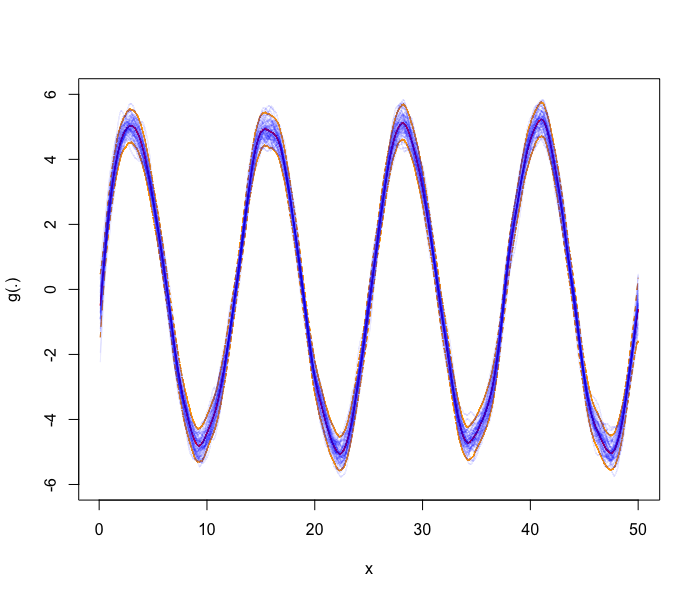
\includegraphics[width=0.47\textwidth]{sim1-function-method1.png}
    }
    \subfigure[Function inferred and interpolated using Method 2]{
      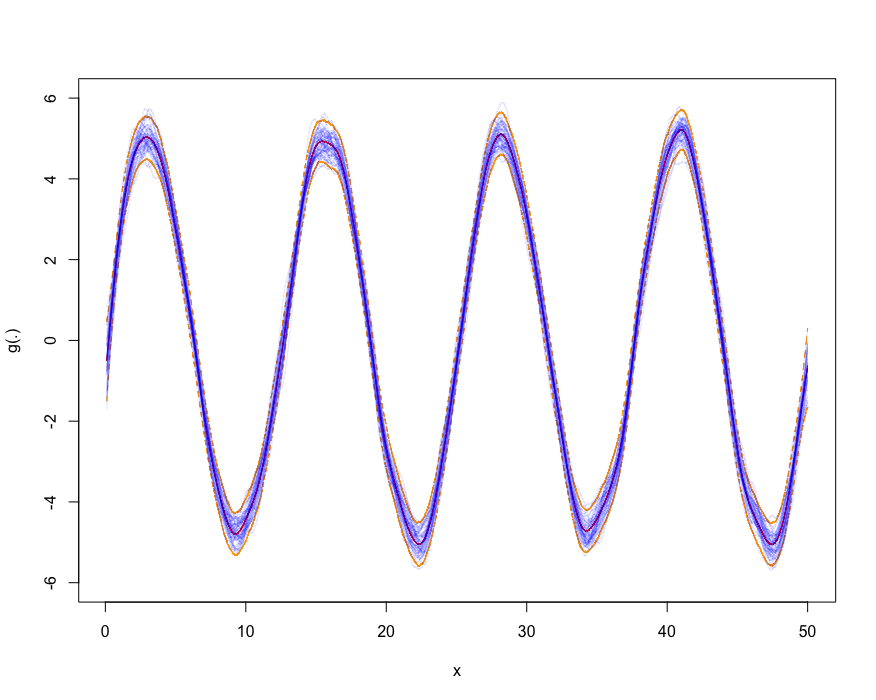
\includegraphics[width=0.47\textwidth]{sim1-function-method2.png}
    }
    \subfigure[Function inferred and interpolated using Method 3 (linear)]{
      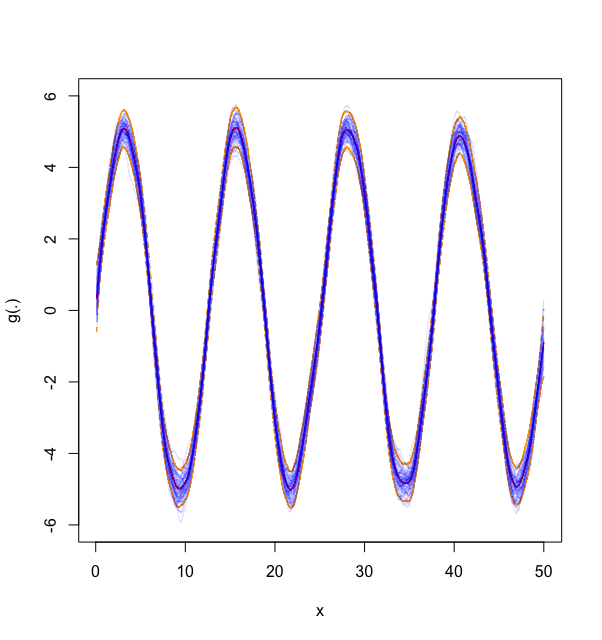
\includegraphics[width=0.47\textwidth]{sim1-function-method3linear.png}
    }
        \subfigure[Function inferred and interpolated using Method 3 (cubic)]{
      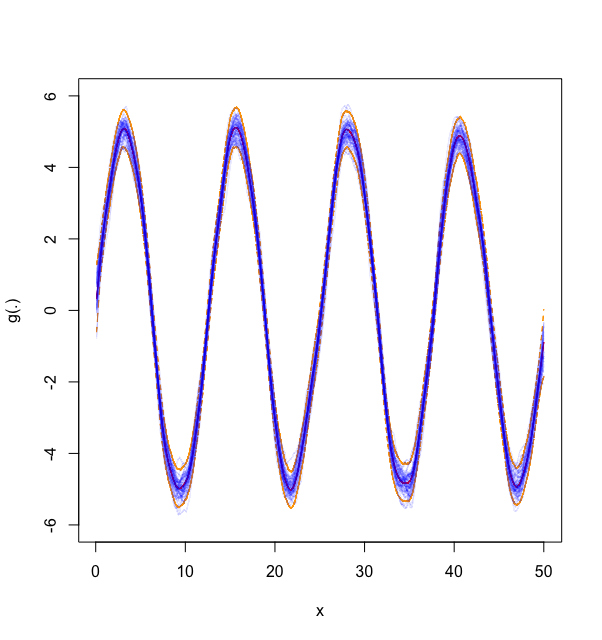
\includegraphics[width=0.47\textwidth]{sim1-function-method3cubic.png}
    }
    \caption{Inference for the function $g(.)$ using different methods; The light blue lines are samples from the posterior distribution; The red lines are posterior mean of the function; The orange lines are the posterior credible interval with 95 percent coverage rate.}
    \label{fig:sim1func}
\end{figure}


Then, using the interpolated functions we can also do inference on the derivative and the second derivative of the function $g(.)$. Although functions interpolated using the linear B spline function will not be differentiable at the knots, the integral of their derivatives can still be defined and computed in ordinary approach. In this case, the computed derivative of linearly interpolated function will be step function that jumps at the knots, and the second derivative will be a constant zero function, with jumps at the knots.

\begin{figure}[p]
    \centering
    \subfigure[First derivative inferred using Method 1]{
      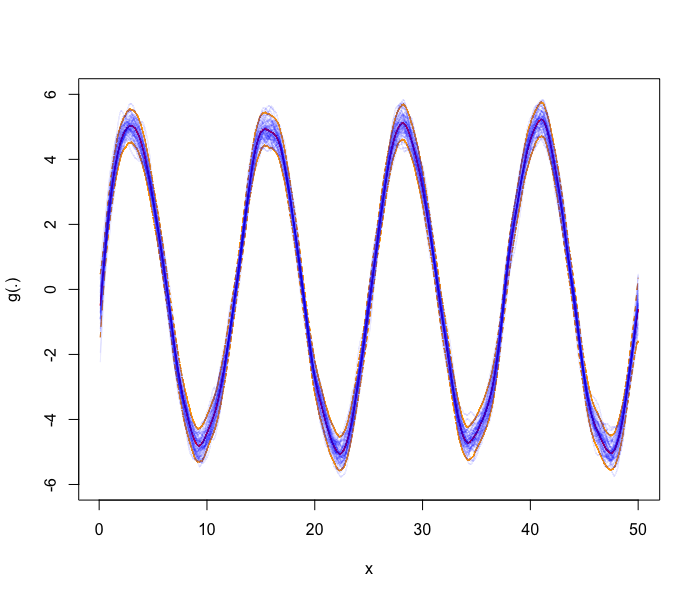
\includegraphics[width=0.47\textwidth]{sim1-function-method1.png}
    }
    \subfigure[First derivative inferred using Method 2]{
      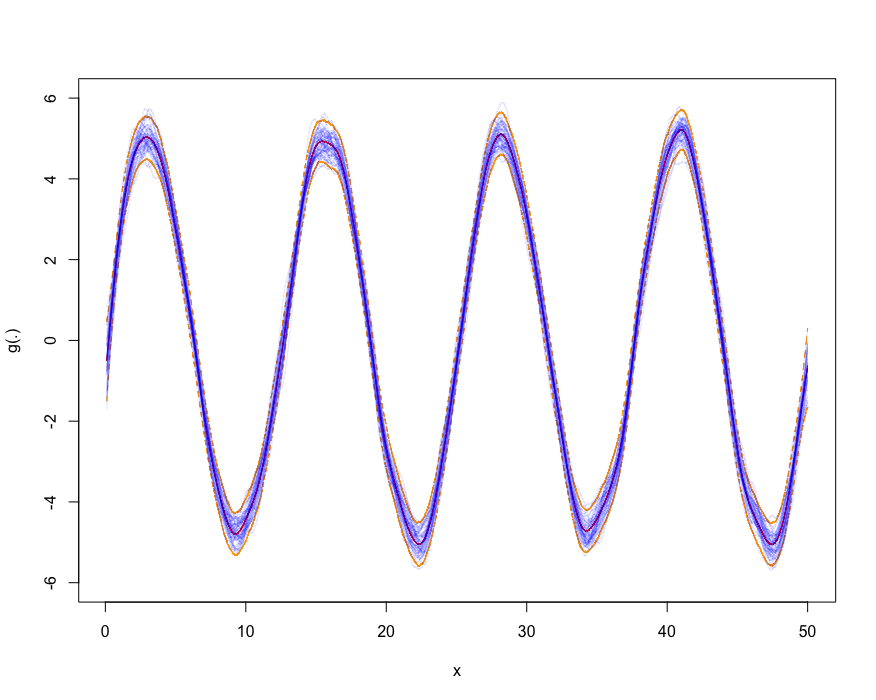
\includegraphics[width=0.47\textwidth]{sim1-function-method2.png}
    }
    \subfigure[First derivative inferred using Method 3 (linear)]{
      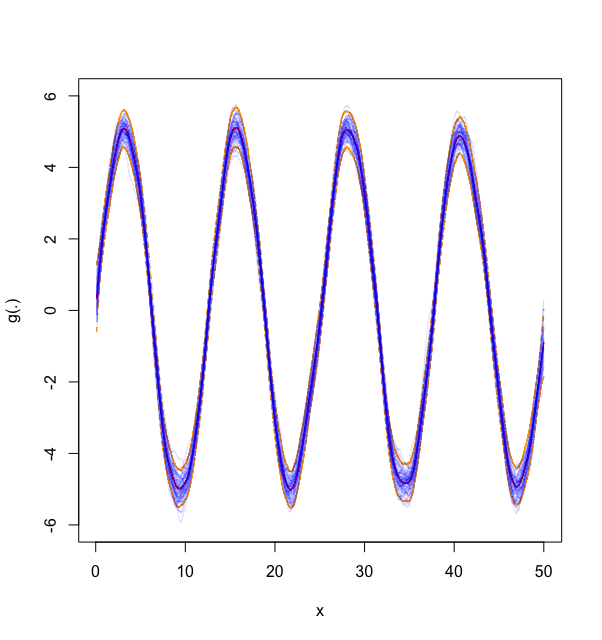
\includegraphics[width=0.47\textwidth]{sim1-function-method3linear.png}
    }
        \subfigure[First derivative inferred using Method 3 (cubic)]{
      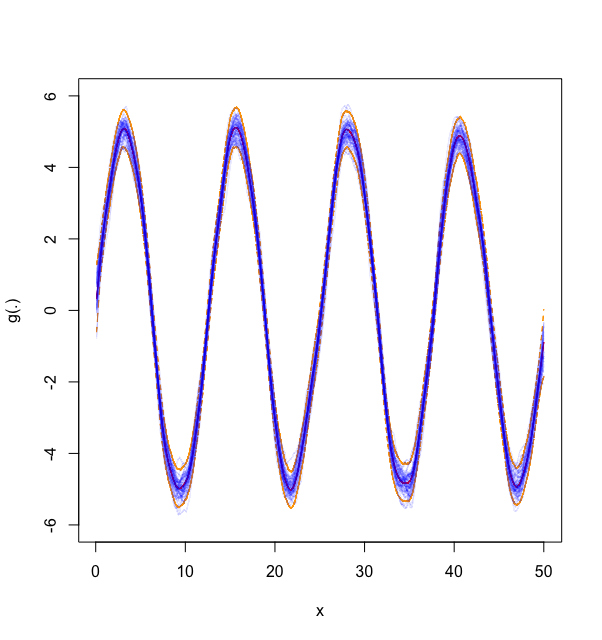
\includegraphics[width=0.47\textwidth]{sim1-function-method3cubic.png}
    }
    \caption{Inference for the function $g'(.)$ using different methods; The light blue lines are samples from the posterior distribution; The red lines are posterior mean of the function; The orange lines are the posterior credible interval with 95 percent coverage rate.}
    \label{fig:sim1func_deriv}
\end{figure}

\begin{figure}[p]
    \centering
    \subfigure[Second derivative inferred using Method 1]{
      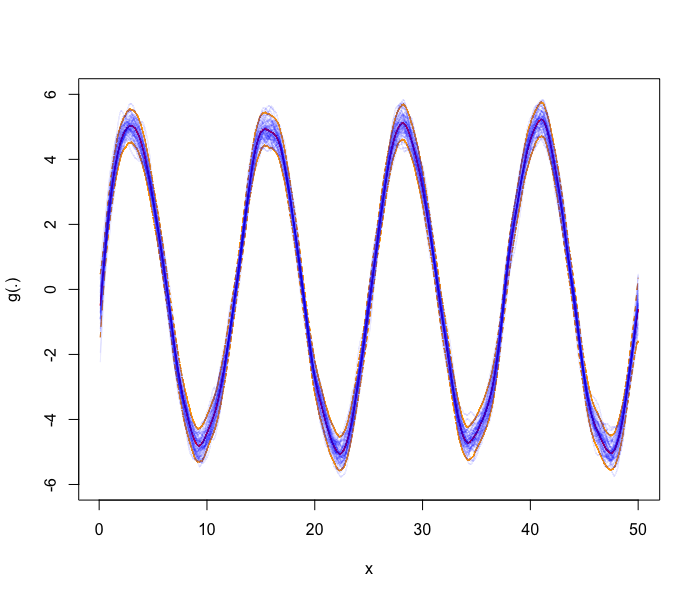
\includegraphics[width=0.47\textwidth]{sim1-function-method1.png}
    }
    \subfigure[Second derivative inferred using Method 2]{
      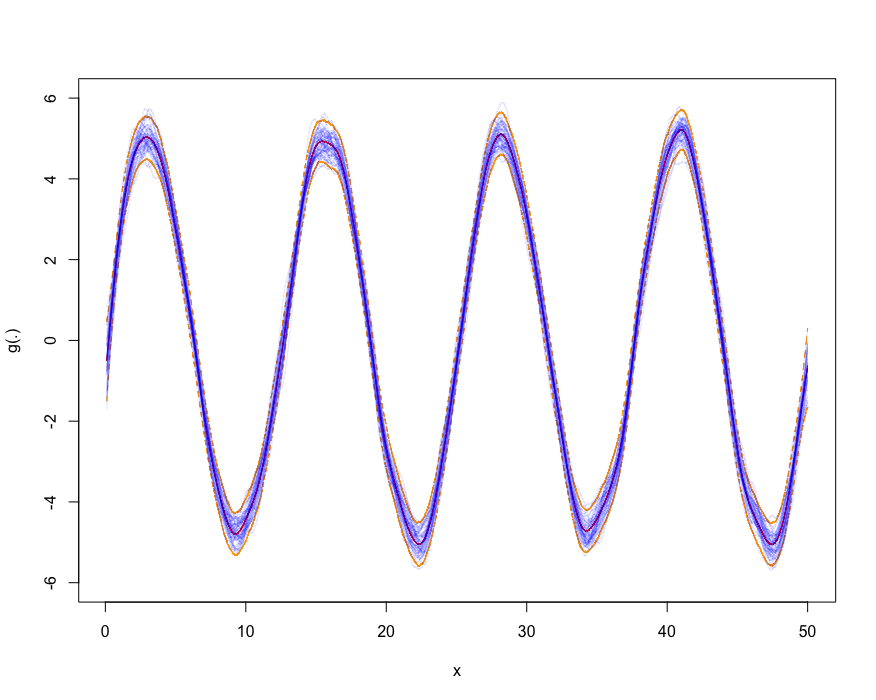
\includegraphics[width=0.47\textwidth]{sim1-function-method2.png}
    }
    \subfigure[Second derivative inferred using Method 3 (linear)]{
      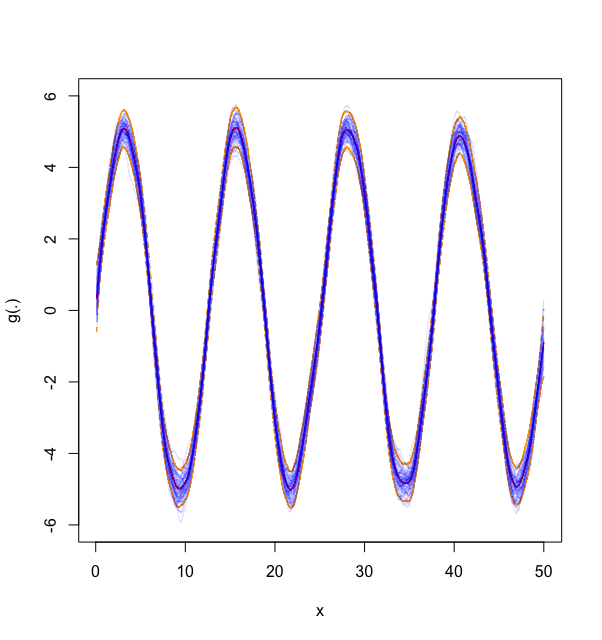
\includegraphics[width=0.47\textwidth]{sim1-function-method3linear.png}
    }
        \subfigure[Second derivative inferred using Method 3 (cubic)]{
      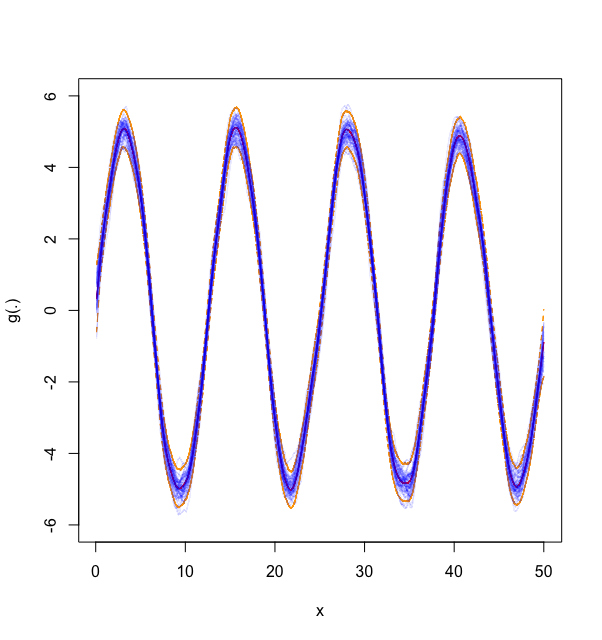
\includegraphics[width=0.47\textwidth]{sim1-function-method3cubic.png}
    }
    \caption{Inference for the function $g''(.)$ using different methods; The light blue lines are samples from the posterior distribution; The red lines are posterior mean of the function; The orange lines are the posterior credible interval with 95 percent coverage rate.}
    \label{fig:sim1func_deriv}
\end{figure}




\section{Conclusion}\label{conclusion}
\ziang{Summarizes the conceptual/practical findings from section 3 and 4.}

\newpage
\bibliographystyle{apalike}
\bibliography{references}




\end{document}